\documentclass[aspectratio=169]{beamer}

\usetheme{Madrid}
\usecolortheme{seahorse}
\setbeamertemplate{navigation symbols}{}
\setbeamertemplate{footline}[frame number]
\setbeamercovered{invisible}

\usepackage[utf8]{inputenc}
\usepackage[T1]{fontenc}
\usepackage{lmodern}
\usepackage{graphicx}
\usepackage{amsmath}
\usepackage{siunitx}
\usepackage{booktabs}
\usepackage{tikz}

\sisetup{separate-uncertainty=true}

\graphicspath{{figures/}{figures/pngs/}{figures/parameter_analysis/}}

\newcommand{\silnit}{\mathrm{SiN}}
\newcommand{\fatu}{\mathbf{u}}
\newcommand{\fatsig}{\boldsymbol{\sigma}}
\newcommand{\fatA}{\mathbf{A}}
\newcommand{\fatM}{\mathbf{M}}
\newcommand{\ngsolve}{%
  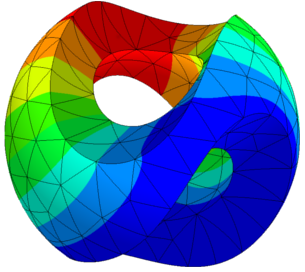
\includegraphics[height=1.25\fontcharht\font`A]{ngsolvelogo.png}%
  \text{NGSolve }%
}
\newcommand{\normalLogoHeight}{0.7cm}
\newcommand{\titleLogoHeight}{1.35cm}
\newcommand{\plotTextMatchScale}{1.10}
\newcommand{\sampleRingRadius}{1.09cm}
\newcommand{\sampleRingThickness}{1.3pt}
\newcommand{\modeShapeWithCenterDot}[1]{%
  \begin{tikzpicture}
    \node[inner sep=0pt] (modeplot) {\includegraphics[width=\linewidth]{#1}};
    \fill[yellow,draw=black,line width=0.35pt] (modeplot.center) circle[radius=0.09cm];
  \end{tikzpicture}%
}
\newcommand{\modeShapeWithCenterRing}[3]{%
  \begin{tikzpicture}
    \node[inner sep=0pt] (modeplot) {\includegraphics[width=\linewidth]{#1}};
    \only<2->{\draw[yellow,line width=#3] (modeplot.center) circle[radius=#2];}
  \end{tikzpicture}%
}

\AddToHook{shipout/foreground}{%
  \begin{tikzpicture}[remember picture,overlay]
    \ifnum\value{framenumber}=1
      \node[anchor=north east, xshift=-0.35cm, yshift=-0.22cm] at (current page.north east)
        {
\includegraphics[height=\titleLogoHeight]{tu-wien-logo-vector.pdf}};
      \node[anchor=north east, xshift=-2.15cm, yshift=-0.22cm] at (current page.north east)
        {
\includegraphics[height=\titleLogoHeight,trim=0 55 0 55,clip]{isas.jpg}};
    \else
      \ifnum\value{framenumber}=\inserttotalframenumber
        \node[anchor=south east, xshift=-0.35cm, yshift=0.55cm] at (current page.south east)
          {
\includegraphics[height=\titleLogoHeight]{tu-wien-logo-vector.pdf}};
        \node[anchor=south east, xshift=-2.15cm, yshift=0.55cm] at (current page.south east)
          {
\includegraphics[height=\titleLogoHeight,trim=0 55 0 55,clip]{isas.jpg}};
      \else
        \node[anchor=north east, xshift=-0.18cm, yshift=-0.07cm] at (current page.north east)
          {
\includegraphics[height=\normalLogoHeight]{tu-wien-logo-vector.pdf}};
        \node[anchor=north east, xshift=-0.95cm, yshift=-0.07cm] at (current page.north east)
          {
\includegraphics[height=\normalLogoHeight,trim=0 55 0 55,clip]{isas.jpg}};
      \fi
    \fi
  \end{tikzpicture}%
}

\title[Mechanical FEM Simulation of Nanomembranes]{Mechanical FEM Simulation of Sampled Nanomembranes for Mass Detection}
\author{Tobias Slowiak}
\institute{Institut f\"ur Sensor- und Aktuatorsysteme, TU Wien}
\date{Master's Thesis Defense}

\begin{document}

\begin{frame}
  \titlepage
\end{frame}

\begin{frame}{Nanoelectromechanical membranes}
  \begin{columns}[T,onlytextwidth]
    \column{0.52\textwidth}
    \begin{itemize}[<+(1)->]
      \item EMILIE is a device for improved Infrared Spectroscopy.
      \item Enables characterization of very small sample masses.
      \item In this context we look at approximately\\$0.6$ - $\SI{40}{\nano\gram}$.
    \end{itemize}
    \begin{block}<+(1)->{Mechanical information}
      This thesis focuses on the \textbf{purely mechanical} response of the EMILIE membranes to deposited samples
      to extract information about the sample.
      \end{block}
    \vspace{0.4cm}
    \column{0.42\textwidth}
    \centering
    \def\emiliePanelWidth{0.75\linewidth}
    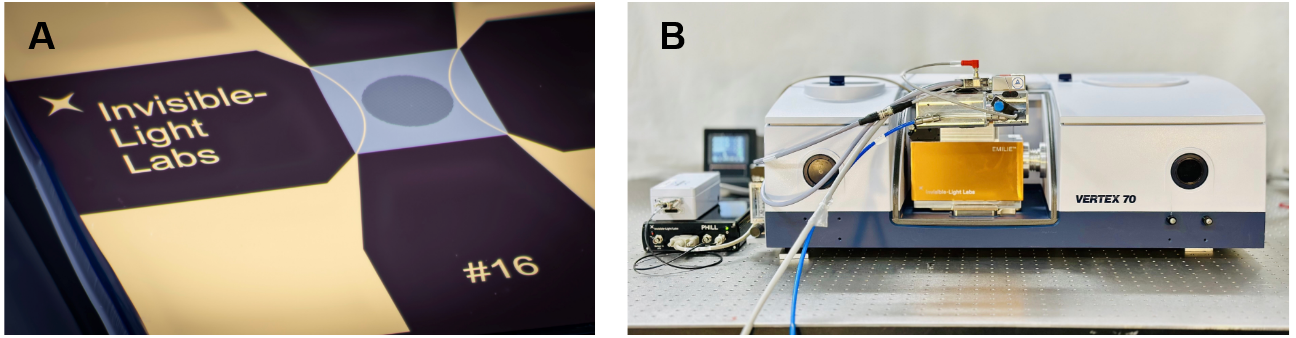
\includegraphics[width=\emiliePanelWidth,trim=0 0 525 0,clip]{EMILIE.png}
    \vspace{0.12cm}

    \makebox[\linewidth][c]{\hspace*{-0.05cm}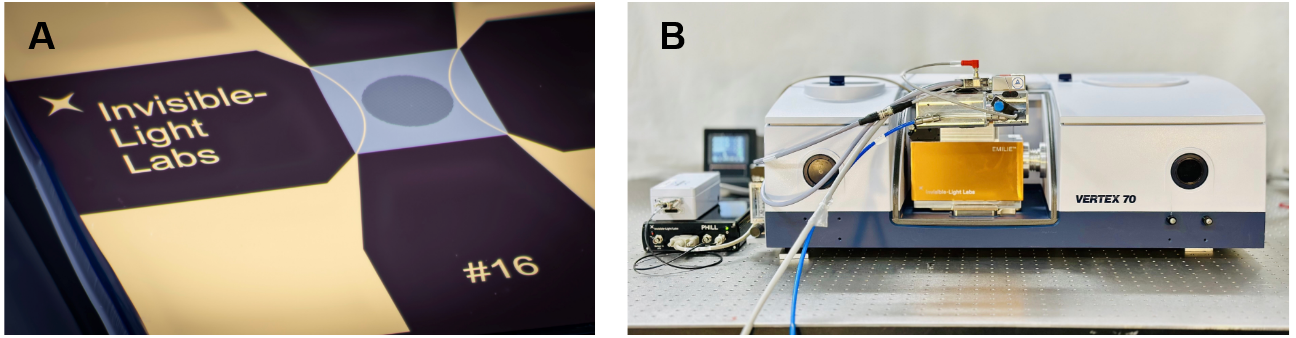
\includegraphics[width=\emiliePanelWidth,trim=475 0 0 0,clip]{EMILIE.png}}
  \end{columns}
\end{frame}

\begin{frame}{Motivation and Problem Statement}
    \begin{enumerate}[<+(1)->]
      \item Previous simulation attempts in \textsc{Comsol} had problems due to element aspect ratios etc.
      \item Smaller computational cost would be desirable for some possible applications.
    \end{enumerate}
    \begin{block}<+(1)->{Main Objective}
      \begin{itemize}[<+->]
        \item Assess whether a purely mechanical simulation can capture the system behavior
        \item Estimate the membrane prestress from the measured response
        \item Evaluate how accurately the sample mass can be inferred from the mechanical response
        \item Evaluate how accurately the sample position can be inferred from the mechanical response
      \end{itemize}
      \uncover<+->{\textbf{Goal:} Build a mechanical FEM model that links deposited mass distributions to measurable resonance frequency shifts.}
    \end{block}
\end{frame}

\begin{frame}{Simulation model}
  \footnotesize
  \setlength{\abovedisplayskip}{0.08cm}
  \setlength{\belowdisplayskip}{0.08cm}
  \begin{columns}[T,onlytextwidth]
    \column{0.62\textwidth}
    \begin{itemize}
      \setlength\itemsep{0pt}
      \item<2-> The membrane is modeled as a two-dimensional prestressed elastic structure.
      \item<3-> Bending stiffness is negligible for the considered modes.
      \item<4-> Two coupled PDEs:
      \begin{itemize}
        \setlength\itemsep{0pt}
        \item<5-> static elasticity for displacement and stress redistribution
            \[
              -\nabla\cdot\fatsig_\fatu = \nabla\cdot\fatsig_p,
            \]
        \item<6-> wave eigenvalue problem for resonance frequencies
        \[
            \nabla \cdot \left( \fatsig(x,y) \cdot \nabla u \right) 
    = \rho \, \frac{\partial^2 u(x,y,t)}{\partial t^2}.
    \]
      \end{itemize}
      \item<7-> The model is implemented in \ngsolve therefore highly parametrizable and efficient (\SI{1}{\second} computational time on a standard laptop).
    \end{itemize}
    \column{0.34\textwidth}
    \begin{minipage}[t][0.76\textheight][b]{\linewidth}
      \begin{block}<5->{Variables}
        \tiny
        \setlength{\parskip}{0.04cm}
        \uncover<5->{$\fatu$: in-plane displacement field.\par}
        \uncover<5->{$\fatsig_\fatu$: elastic stress caused by $\fatu$.\par}
        \uncover<5->{$\fatsig_p$: prescribed prestress tensor.\par}
        \uncover<6->{$u(x,y,t)$: transverse vibration displacement.\par}
        \uncover<6->{$\fatsig(x,y)$: redistributed membrane stress.\par}
        \uncover<6->{$\rho$: effective mass density.\par}
        \uncover<6->{$x,y,t$: coordinates and time.\par}
      \end{block}
    \end{minipage}
  \end{columns}
\end{frame}

\begin{frame}{Computational domain}
  \begin{columns}[T,onlytextwidth]
    \column{0.48\textwidth}
    \centering
    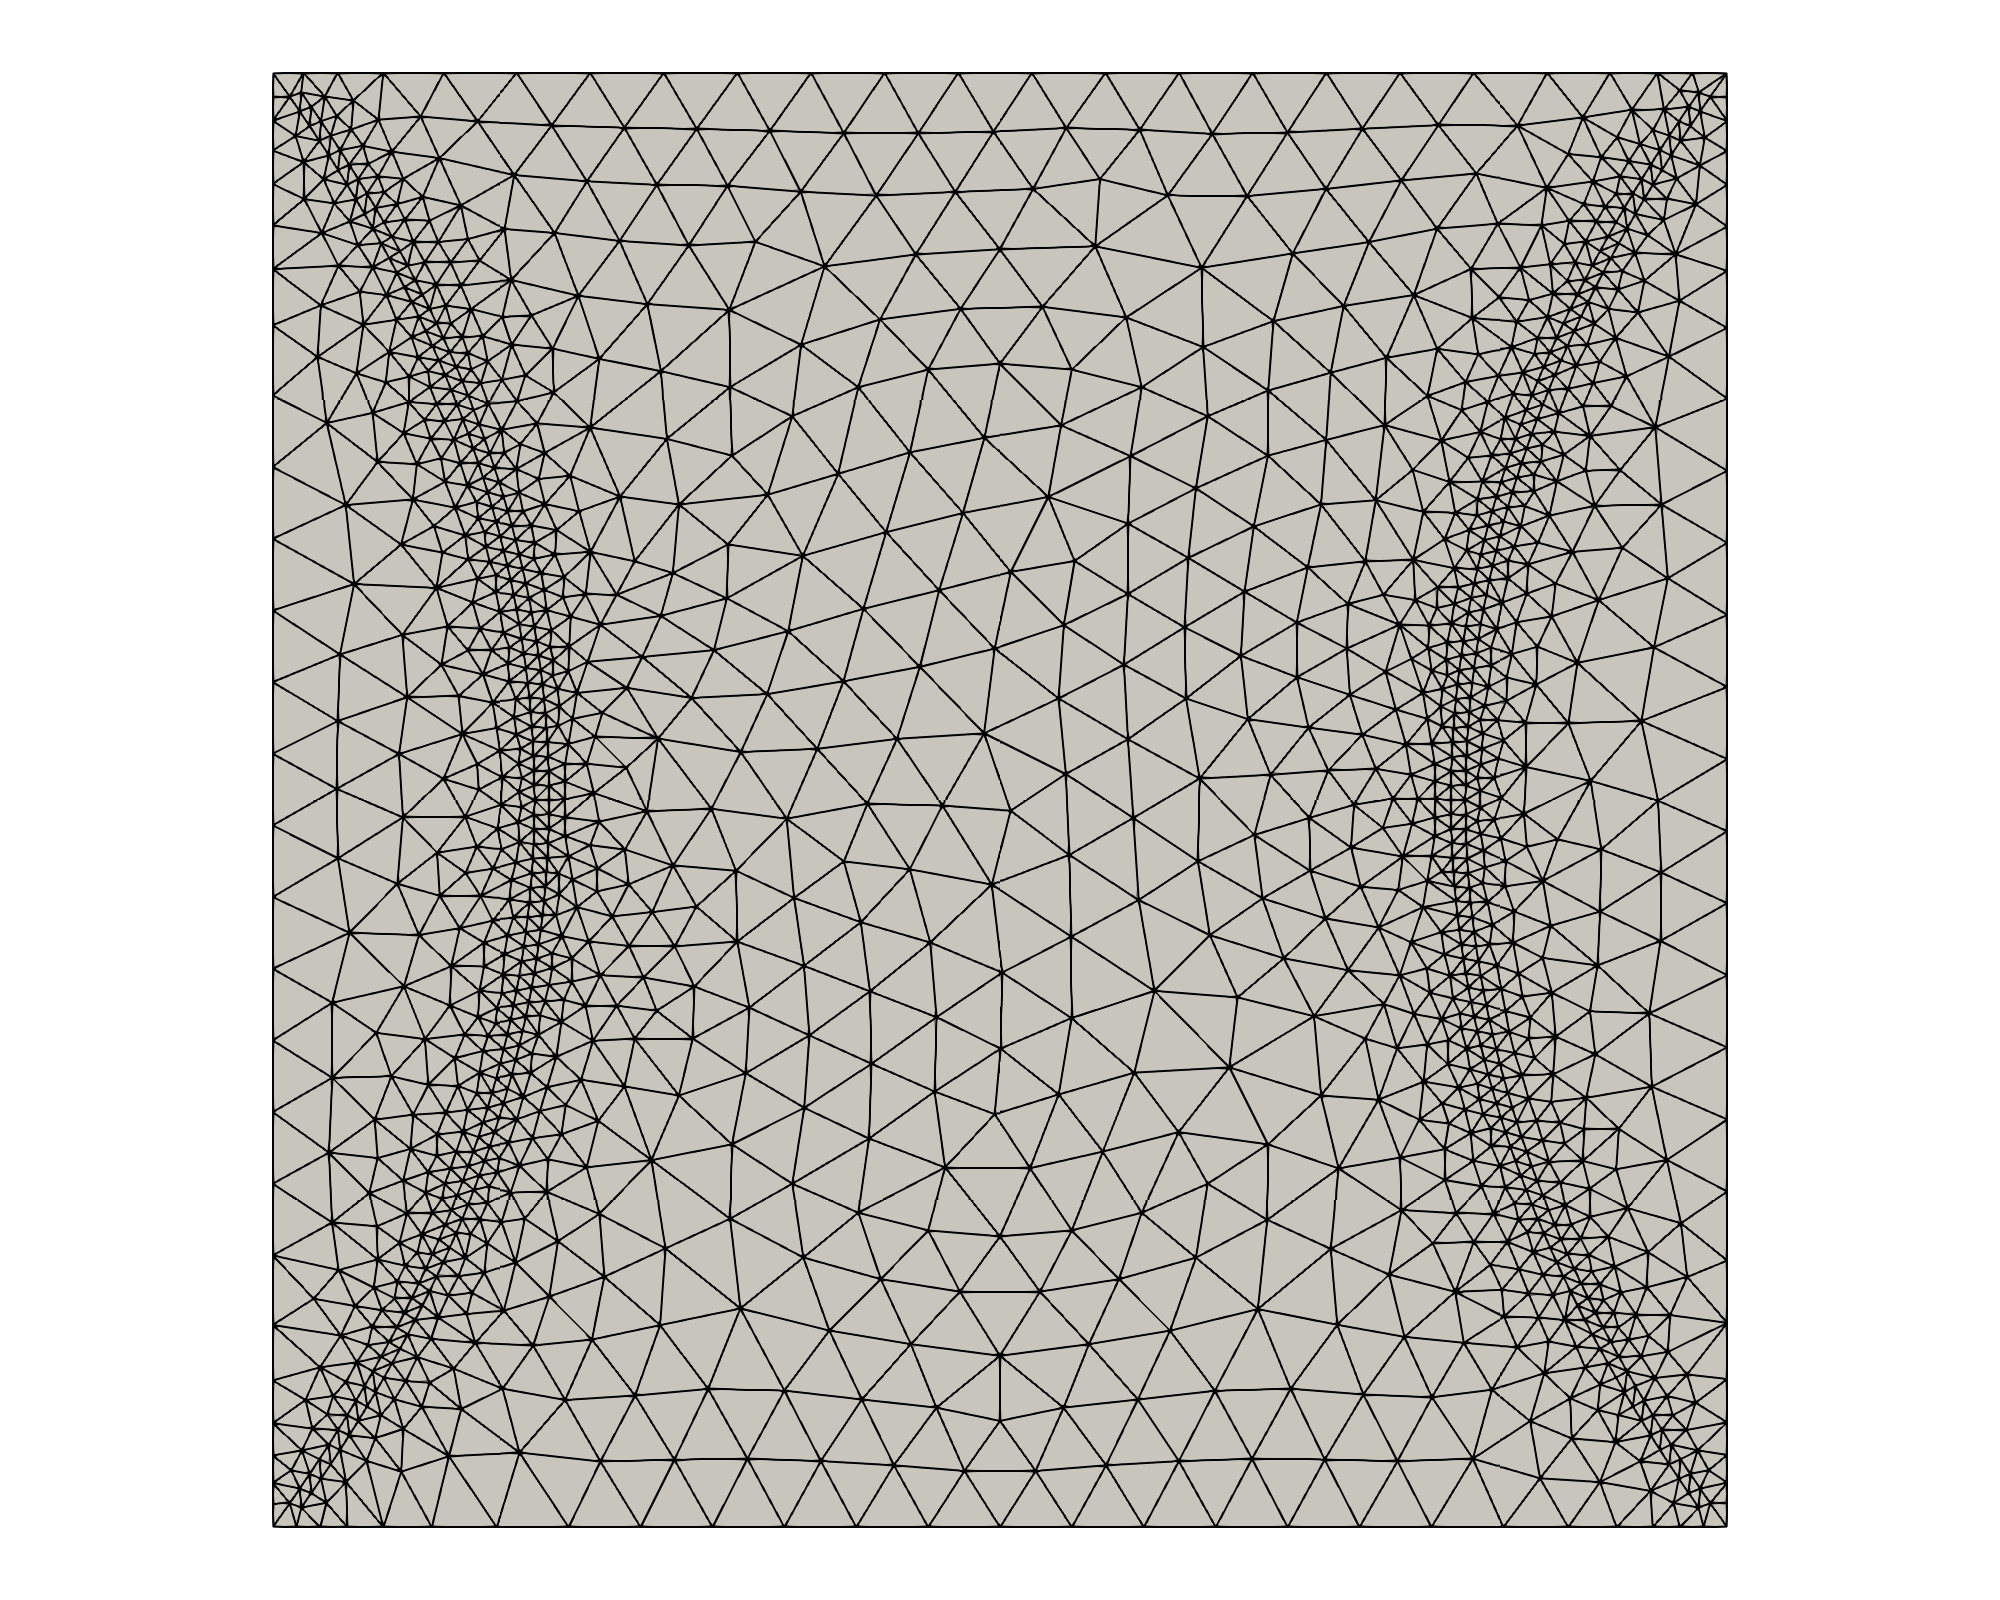
\includegraphics[height=0.55\textheight,trim=260 70 260 70,clip]{mesh.png}
    \column{0.48\textwidth}
    \centering
    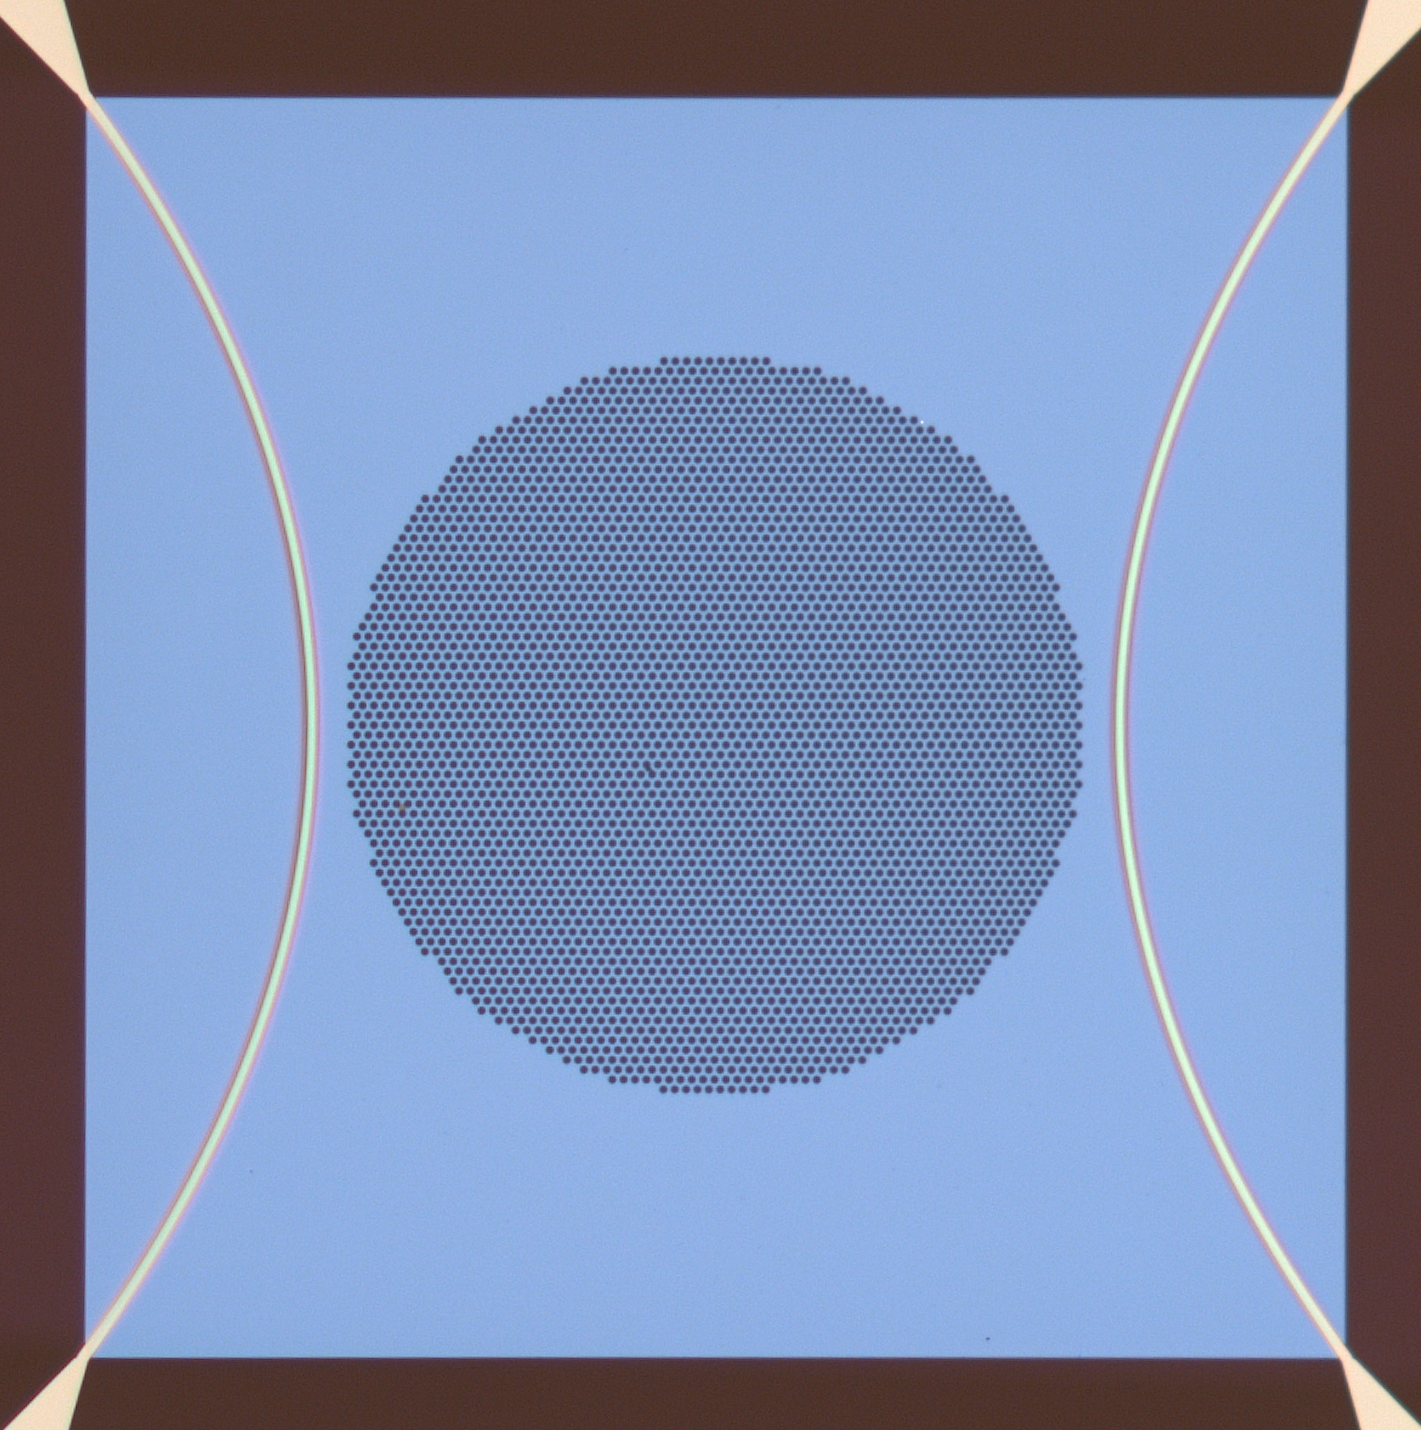
\includegraphics[height=0.55\textheight]{empty_membrane.png}
  \end{columns}
  \vspace{0.25cm}
  \begin{itemize}[<+(1)->]
    \item Perforation modeled by effective density and effective prestress.
    \item Electrodes included through geometry, mass, and prestress.
    \item Sample deposits also resolved in the mesh, shown later.
  \end{itemize}
\end{frame}

\begin{frame}{Prestress estimation}
  \centering
  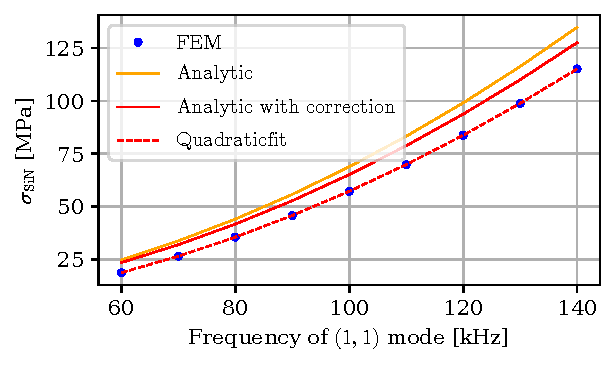
\includegraphics[scale=\plotTextMatchScale]{prestress_estimator_with_corr.pdf}
  \vspace{-0.05cm}

  \begin{itemize}[<+(1)->]
    \setlength\itemsep{0pt}
    \item The model allows for an improved estimate of the prestress, which is in use now.
  \end{itemize}
\end{frame}


\begin{frame}{Mode shapes}
  \begin{columns}[T,onlytextwidth]
    \column{0.33\textwidth}
    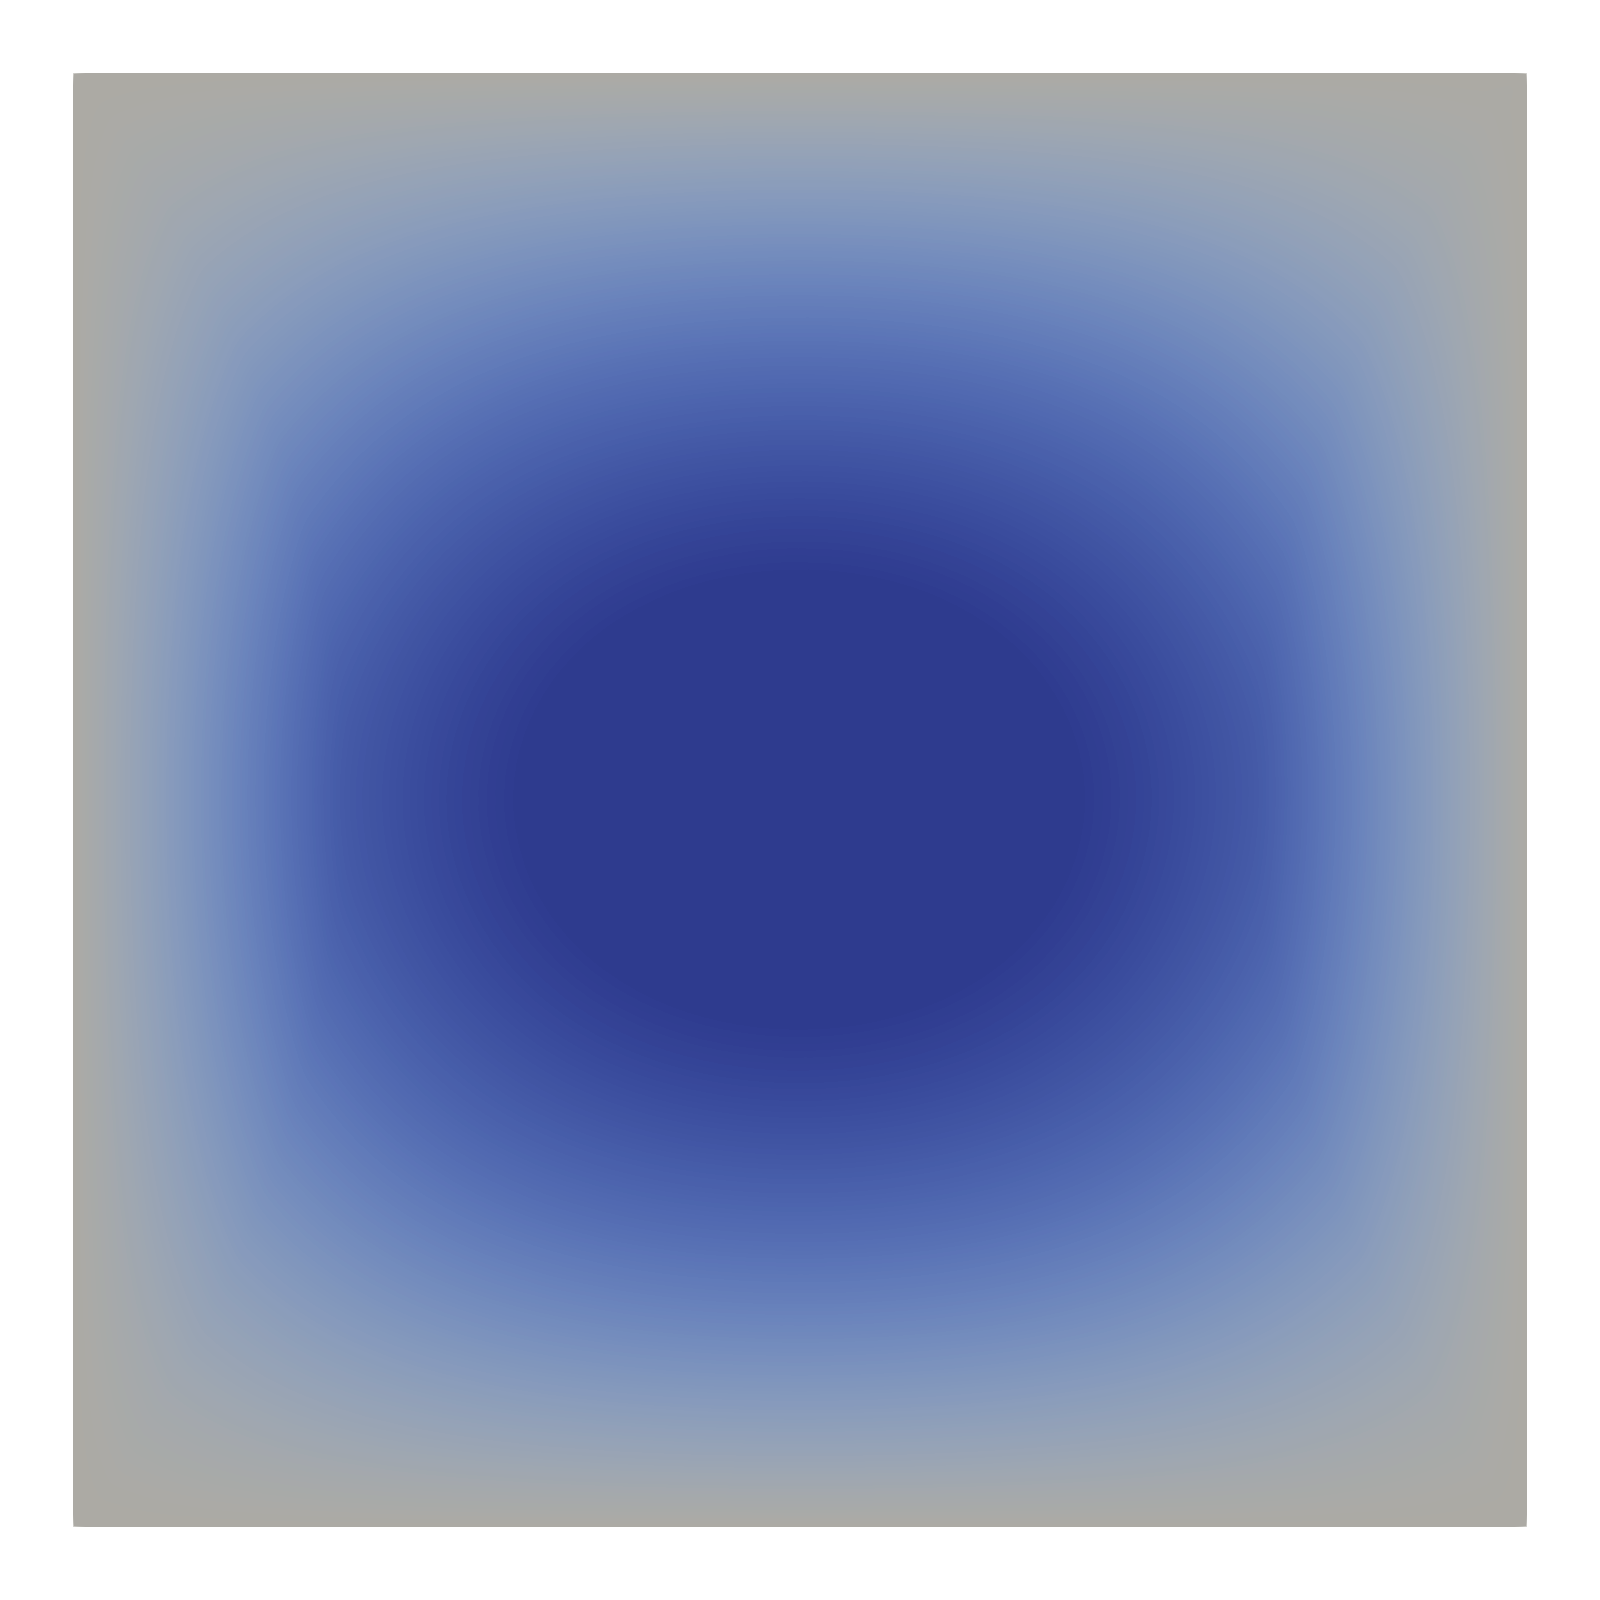
\includegraphics[width=\linewidth]{modeshape_(1,1).png}
    \centering $(1,1)$
    \column{0.33\textwidth}
    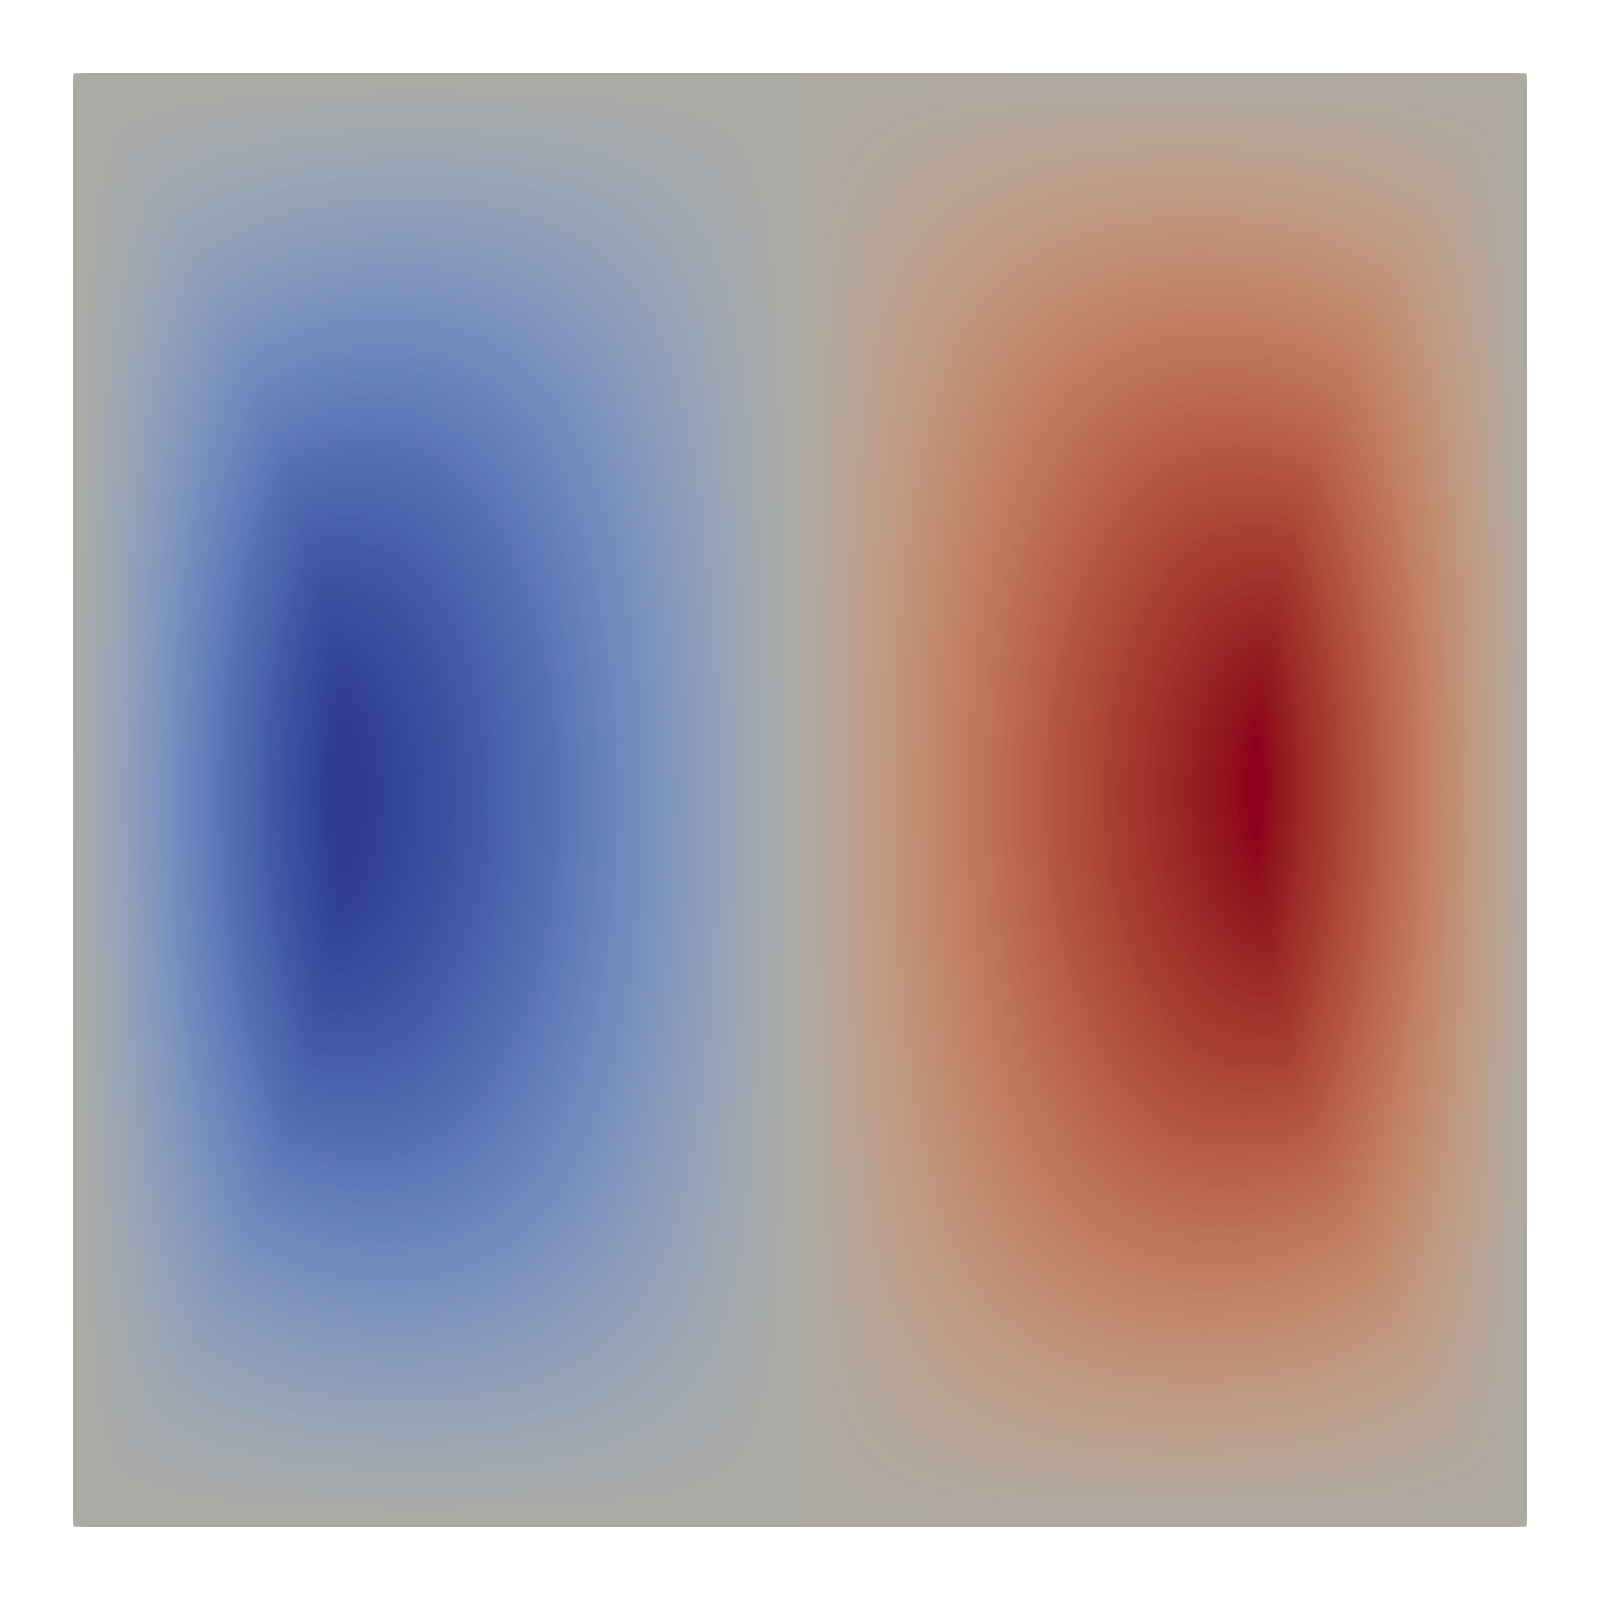
\includegraphics[width=\linewidth]{modeshape_(2,1).png}
    \centering $(2,1)$
    \column{0.33\textwidth}
    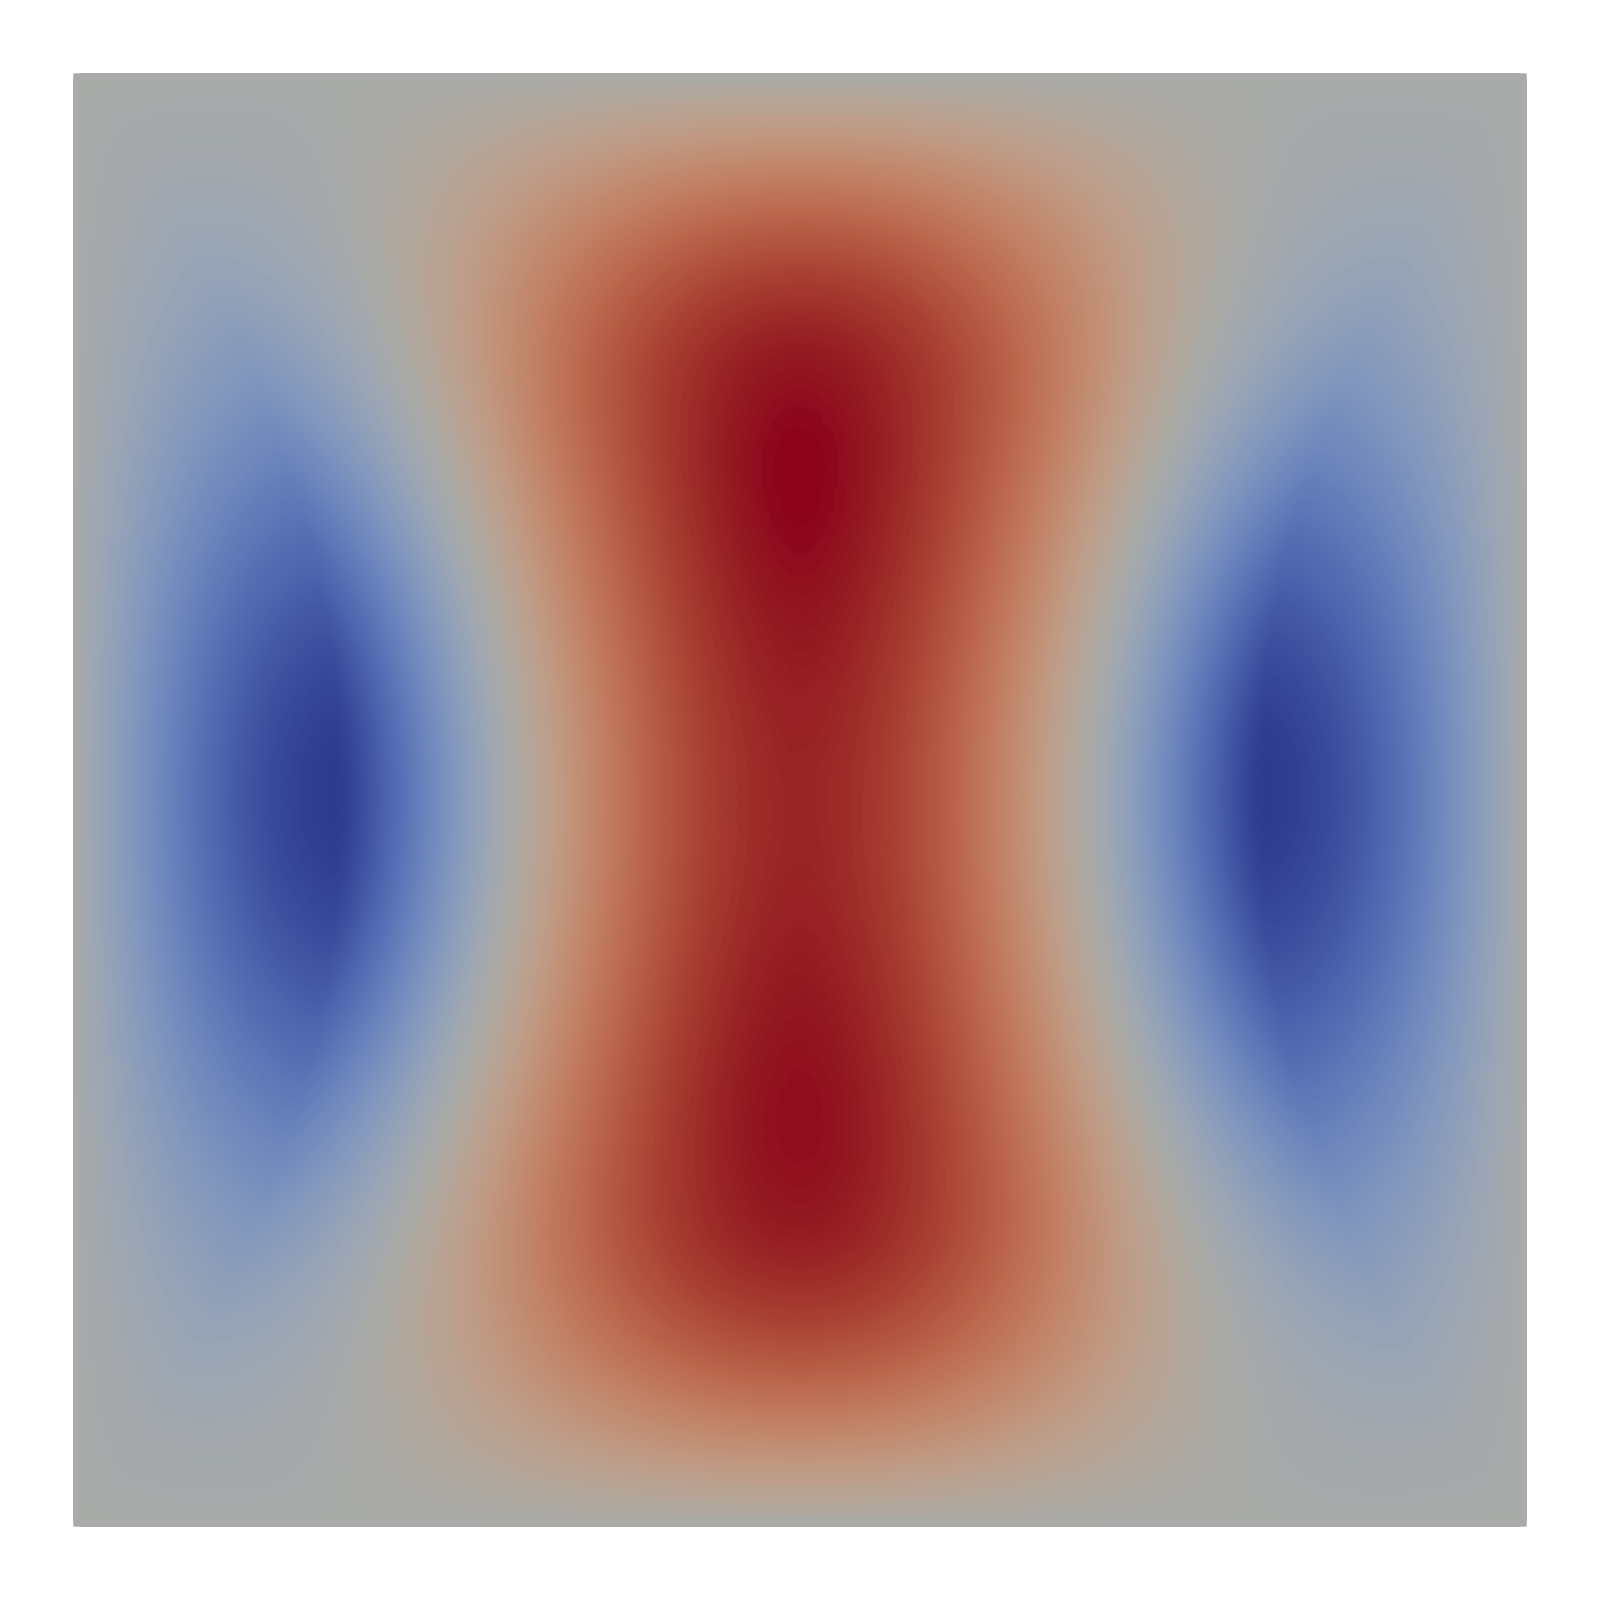
\includegraphics[width=\linewidth]{modeshape_(3,1).png}
    \centering $(3,1)$
  \end{columns}
  \vspace{0.35cm}
  \begin{itemize}[<+(1)->]
    \item Multiple Eigenfrequencies can be measured and simulated, one for each mode shape.
  \end{itemize}
\end{frame}

\begin{frame}{Position detection}
  \begin{columns}[T,onlytextwidth]
    \column{0.33\textwidth}
    \modeShapeWithCenterDot{modeshape_(1,1).png}
    \centering $(1,1)$
    \column{0.33\textwidth}
    \modeShapeWithCenterDot{modeshape_(2,1).png}
    \centering $(2,1)$
    \column{0.33\textwidth}
    \modeShapeWithCenterDot{modeshape_(3,1).png}
    \centering $(3,1)$
  \end{columns}
  \vspace{0.35cm}
  \begin{itemize}[<+(1)->]
    \item Different modes overlap differently with the deposited mass.
    \item From the relative frequency shifts of different modes, the sample position can be inferred.
  \end{itemize}
\end{frame}

\begin{frame}{Coffee-ring samples}
  \centering
  \includegraphics[scale=0.4,trim=0 6 0 6,clip]{pngs/coffeering.png}
  \vspace{-0.05cm}
  \begin{itemize}[<+(1)->]
    \item Sampes are deposited in in solvent droplets.
    \item As the solvent evaporates, the sampled material remains mostly on the rim of the droplet.
  \end{itemize}
\end{frame}

\begin{frame}{Coffee-ring samples}
  \begin{columns}[T,onlytextwidth]
    \column{0.33\textwidth}
    \modeShapeWithCenterRing{modeshape_(1,1)_sampled.png}{\sampleRingRadius}{\sampleRingThickness}
    \centering $(1,1)$
    \column{0.33\textwidth}
    \modeShapeWithCenterRing{modeshape_(2,1)_sampled.png}{\sampleRingRadius}{\sampleRingThickness}
    \centering $(2,1)$
    \column{0.33\textwidth}
    \modeShapeWithCenterRing{modeshape_(3,1)_sampled.png}{\sampleRingRadius}{\sampleRingThickness}
    \centering $(3,1)$
  \end{columns}

\end{frame}

\begin{frame}{Validation: Unsampled membranes}
  \begin{columns}[T,onlytextwidth]
    \column{0.38\textwidth}
    \begin{itemize}[<+(1)->]
      \item Membrane prestress is fitted using the $(1,1)$ mode.
      \item Higher modes are then predicted by the same mechanical model.
      \item Agreement is within experimental error bounds for a broad parameter range.
    \end{itemize}
    \vspace{0.15cm}
    \begin{block}<+(1)->{Good News}
      The model accurately reproduces the measured eigenfrequencies of unsampled membranes, which is a prerequisite for mass detection.
    \end{block}
    \column{0.58\textwidth}
    \centering
    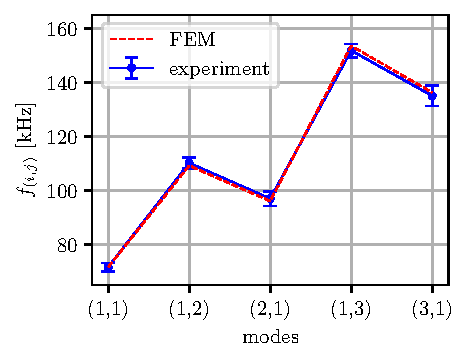
\includegraphics[scale=\plotTextMatchScale]{para_ana_standard.pdf}
  \end{columns}
\end{frame}

\begin{frame}{Validation for other parameters}
  \centering
  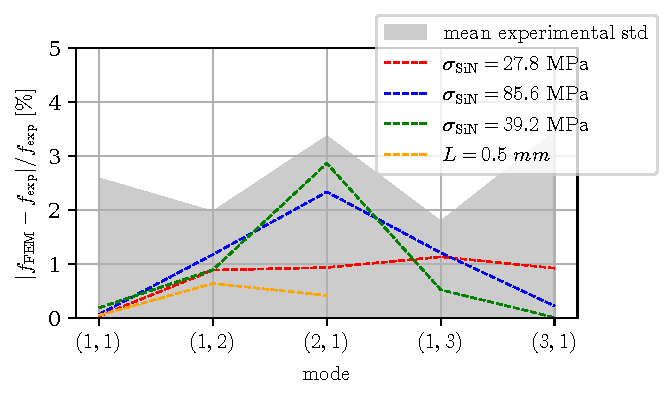
\includegraphics[scale=1.05,trim=0 6 0 6,clip]{other_parameters_mean_abs_fem_exp_difference.pdf}
  \vspace{-0.05cm}

  \begin{itemize}[<+(1)->]
    \setlength\itemsep{0pt}
    \item Across a broad parameter range, the simulation results are within the experimental error bounds.
  \end{itemize}
\end{frame}

\begin{frame}{Polystyrene: Measurement}
  \centering
  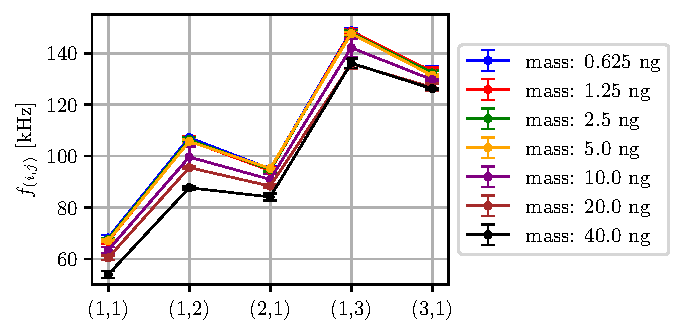
\includegraphics[scale=\plotTextMatchScale]{exp_freqs_sampled_PS.pdf}
  \vspace{-0.05cm}

  \begin{itemize}[<+(1)->]
    \setlength\itemsep{0pt}
    \item PS deposits from \SI{625}{\pico\gram} to \SI{40}{\nano\gram} show measurable frequency shifts.
  \end{itemize}
\end{frame}

\begin{frame}{Polystyrene: Raw simulation data}
  \centering
  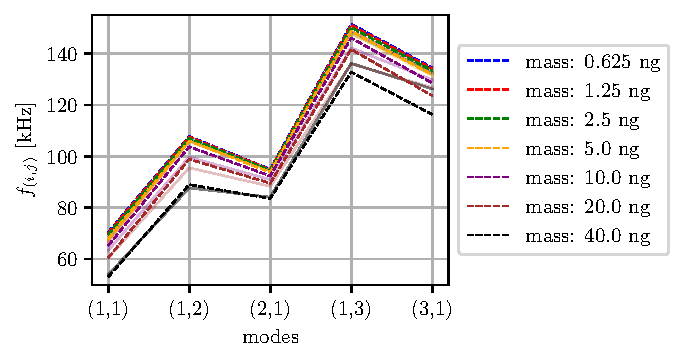
\includegraphics[scale=\plotTextMatchScale]{fem_freqs_sampled_PS.pdf}
  \vspace{-0.05cm}

  \begin{itemize}[<+(1)->]
    \setlength\itemsep{0pt}
    \item Trends are reproduced qualitatively.
  \end{itemize}
\end{frame}


\begin{frame}{Polystyrene: Mass estimation and limits}
  \begin{columns}[T,onlytextwidth]
    \column{0.28\textwidth}
    \begin{itemize}[<+(1)->]
      \setlength\itemsep{0.15cm}
      \item Ideal mass resolution: $\Delta m_\mathrm{ideal} \approx \pm \SI{1.25}{\nano\gram}$.
      \item Current practical accuracy: $\Delta m_\mathrm{current} \approx \pm \SI{5}{\nano\gram}$.
    \end{itemize}
    \column{0.68\textwidth}
    \centering
    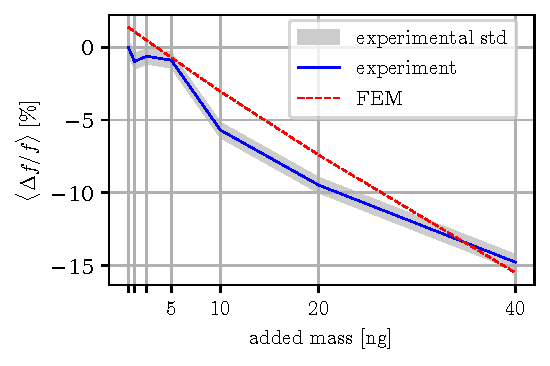
\includegraphics[scale=\plotTextMatchScale]{rel_freq_shift_sampled.pdf}
  \end{columns}
\end{frame}

\begin{frame}{Polystyrene: Model error}
  \centering
  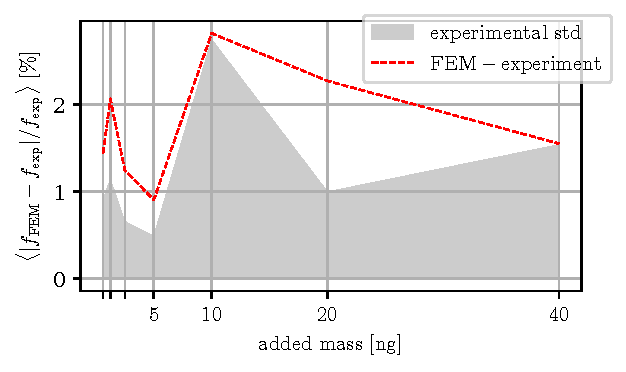
\includegraphics[scale=\plotTextMatchScale]{mean_abs_fem_exp_difference_sampled.pdf}
  \vspace{-0.05cm}

\end{frame}

\begin{frame}{Polypropylene: Measurement}
  \centering
  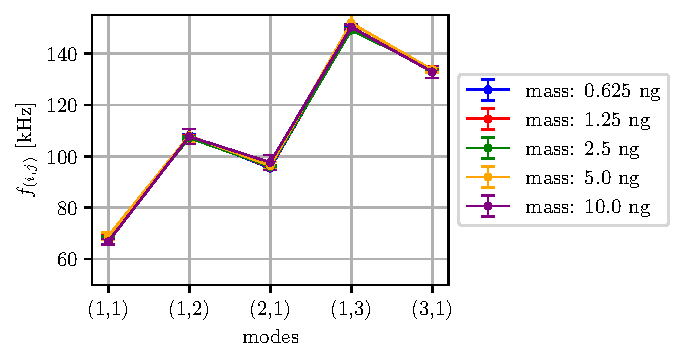
\includegraphics[scale=\plotTextMatchScale]{exp_freqs_sampled_PP.pdf}
  \vspace{-0.05cm}

  \begin{itemize}[<+(1)->]
    \setlength\itemsep{0pt}
    \item PP deposits show almost no systematic frequency decrease with increasing mass.
    \item Added mass alone cannot explain the measurements.
  \end{itemize}
\end{frame}

\begin{frame}{Polypropylene: Model error with sample prestress}
  \begin{columns}[T,onlytextwidth]
    \column{0.5\textwidth}
    \centering
    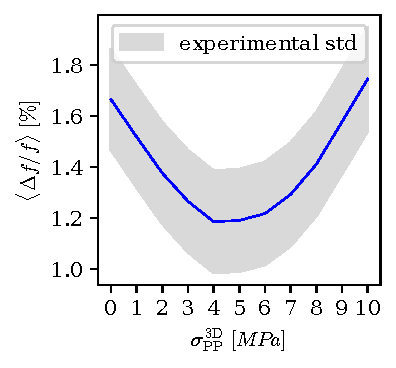
\includegraphics[scale=\plotTextMatchScale]{sample_prestress_analysis.pdf}
    \column{0.35\textwidth}
    \begin{itemize}[<+(1)->]
      \item Agreement improves when internal prestress in the PP deposit is introduced.
    \end{itemize}
    \vspace{0.25cm}
    \begin{block}<+(1)->{Consequence}
      Eigenfrequency shifts can be masked or even reversed by sample prestress.
    \end{block}
  \end{columns}
\end{frame}


\begin{frame}{Conclusions}
  \begin{itemize}[<+(1)->]
    \item A two-dimensional FEM framework for sampled nanomembranes was developed in \ngsolve.
    \item Unsampled membranes are reproduced within experimental uncertainty after prestress fitting.
    \item Mass prediction is feasible for sufficiently large PS samples, roughly above \SI{10}{\nano\gram}.
    \item Mass prediction is limited for small masses and for materials with significant sample prestress.
  \end{itemize}
\end{frame}

\begin{frame}
  \centering
  \Huge Thank you

  \vspace{0.6cm}
  \Large Questions?
\end{frame}

\begin{frame}{MSA Vibrometer}
  \centering
  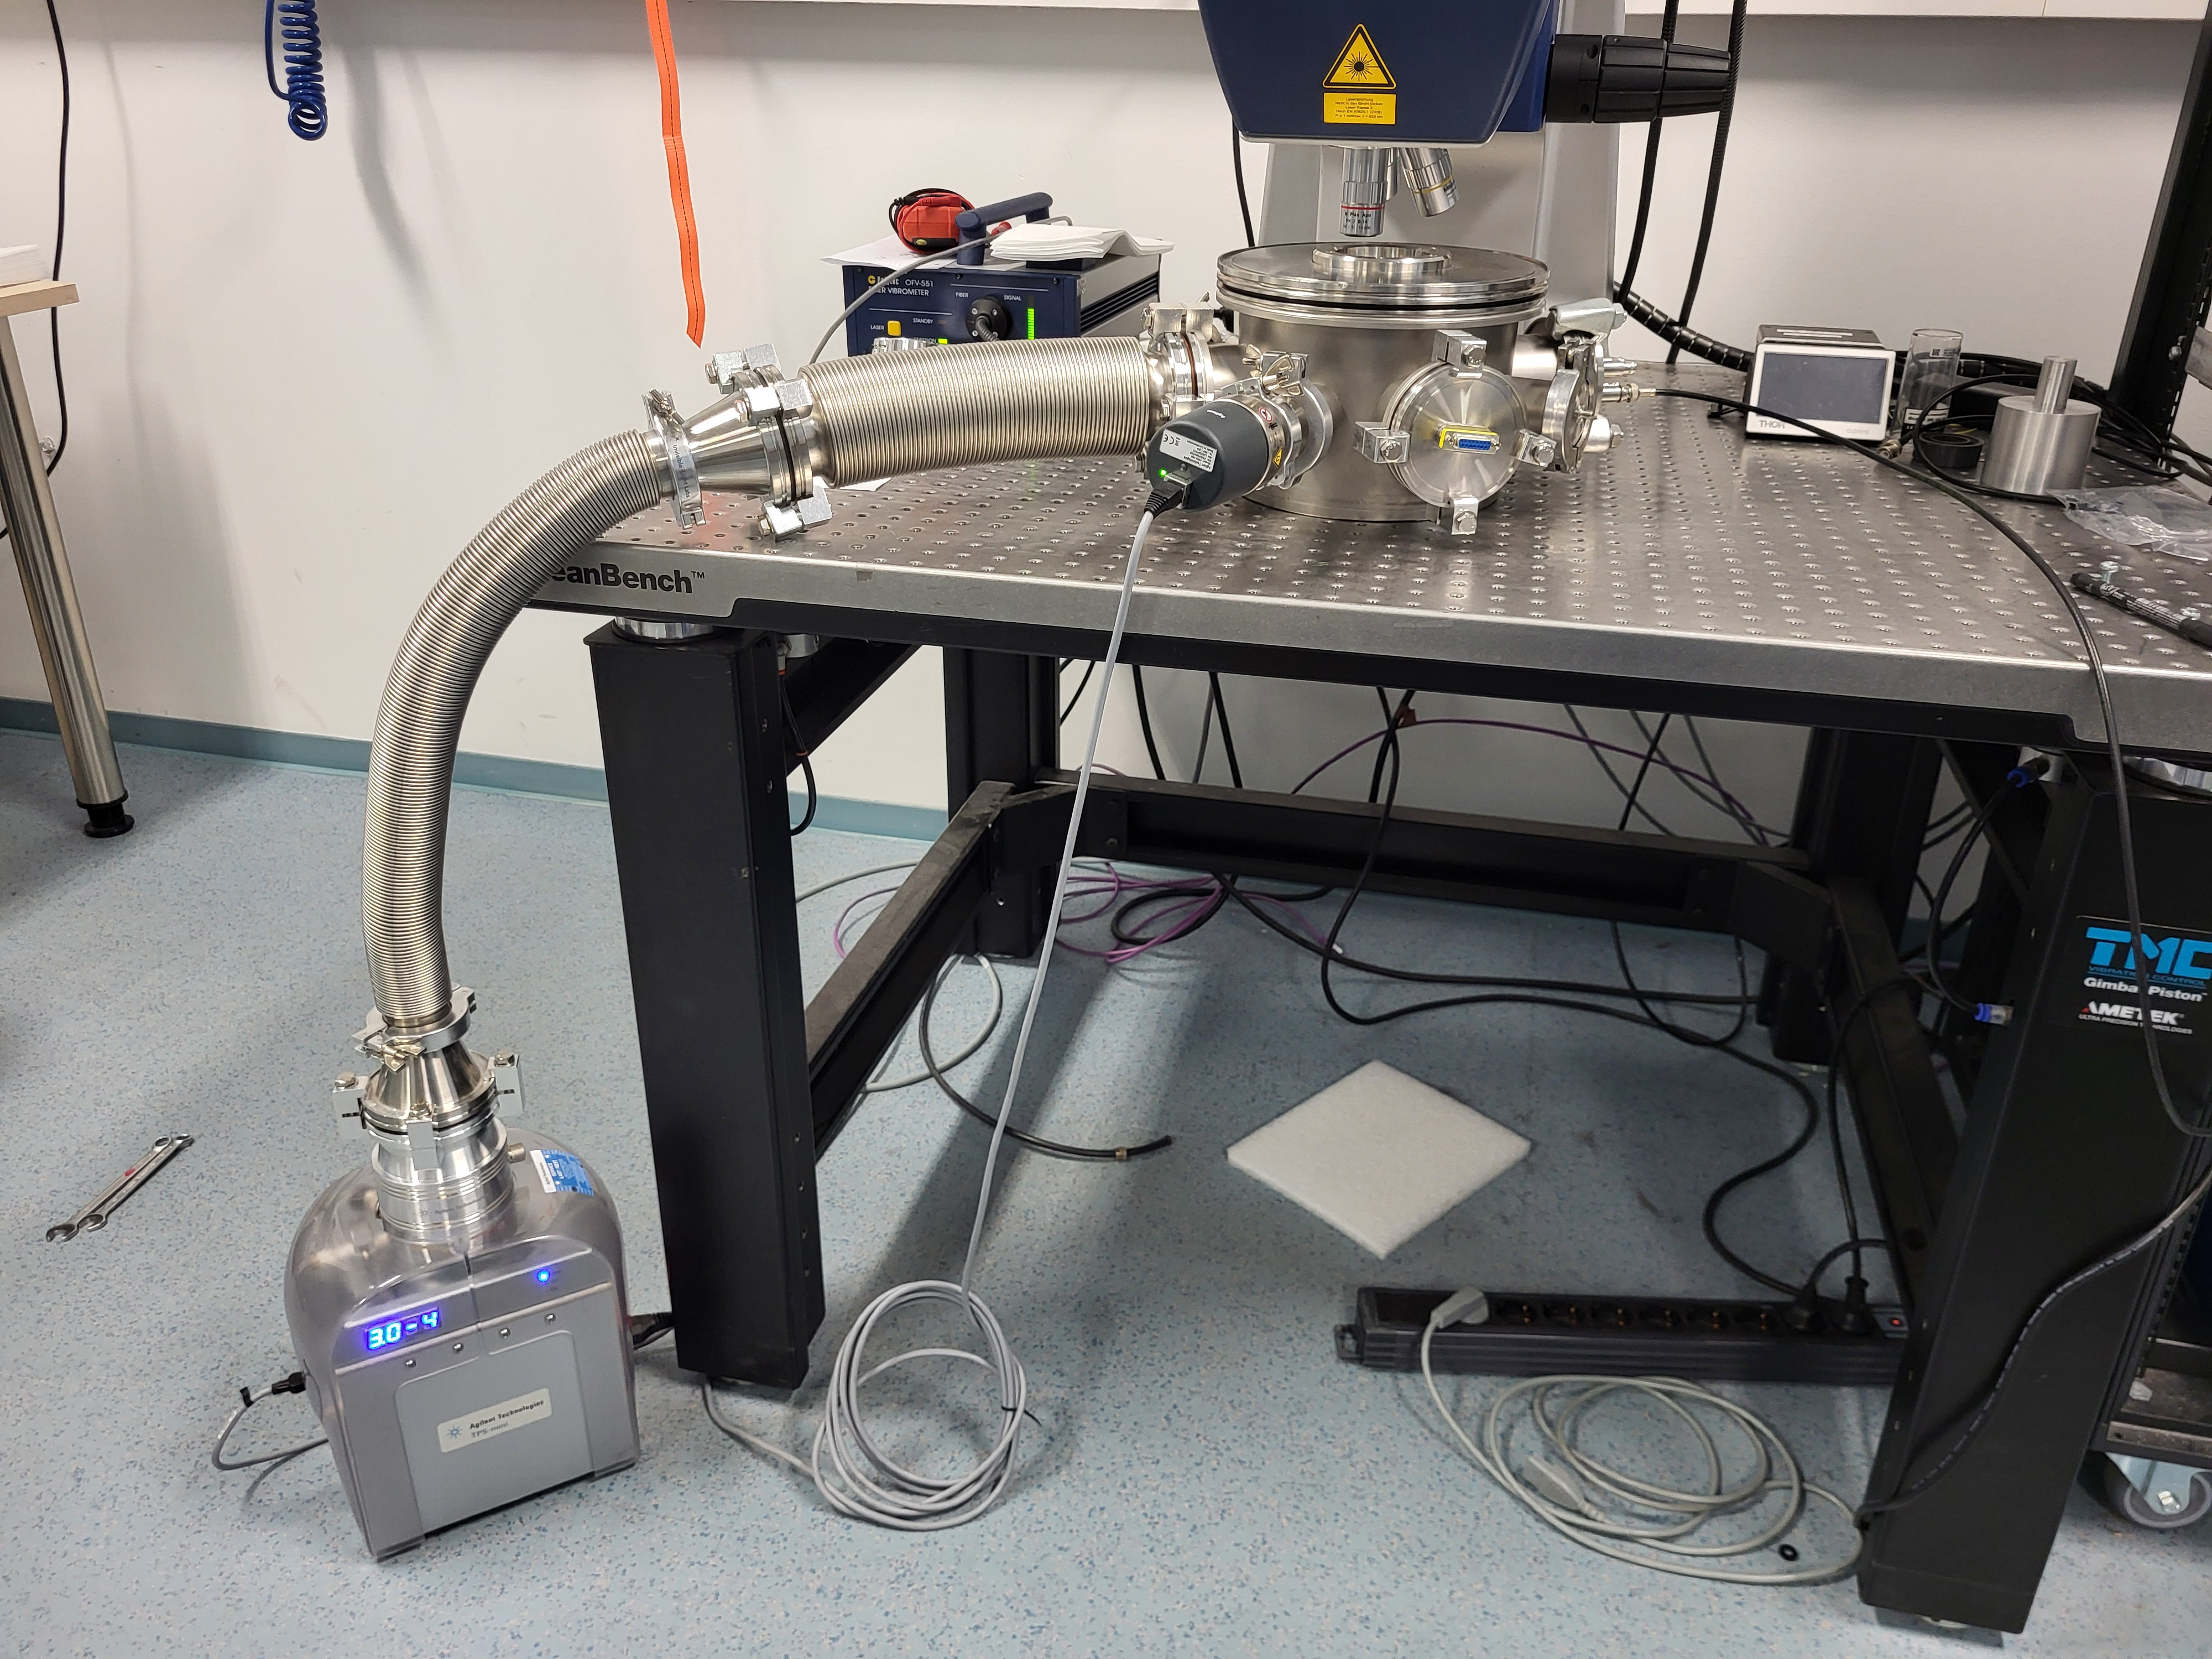
\includegraphics[scale = 0.07]{pngs/MSA_Vibrometer.jpg}
  \vspace{-0.05cm}

\end{frame}

\begin{frame}{Nanobeads}
  \centering
  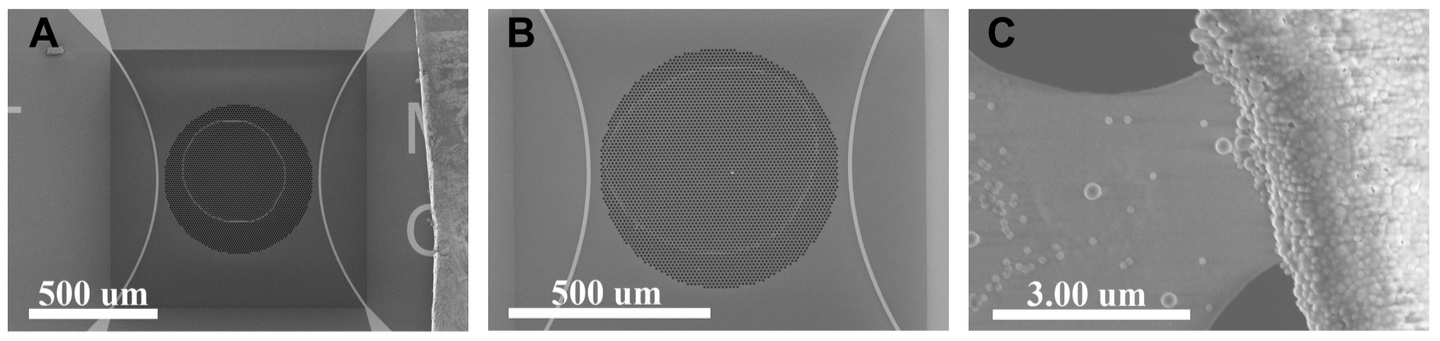
\includegraphics[width=\linewidth]{pngs/Nanobeads.png}
  \vspace{-0.05cm}

\end{frame}

\begin{frame}{Influence of the bending stiffness}
  Assume a homogeneous membrane described by the following PDE:
  \begin{equation}
    \sigma \nabla^2 u + D_p \nabla^4 u - \frac{\partial^2 u}{\partial t^2} = 0.
    \label{eq:kirchhoff_wave}
\end{equation}
  The eigenfrequency found with \SI{25}{\mega\pascal} is
\[
\omega_{31} \approx \SI{9.1e5}{\per\second}.
\] 
Repeating the calculation while omitting the bending term yields 
\[
\omega_{31,\mathrm{nb}} \approx \SI{9.1e5}{\per\second}.
\] 
The relative difference is
\[
\frac{|\omega_{31} - \omega_{31,\mathrm{nb}}|}{\omega_{31}} \approx 5.4 \cdot 10^{-12}.
\]

\end{frame}

\end{document}
